\documentclass{beamer}

\usetheme{Montpellier}
\usecolortheme{rose}

\usepackage[utf8]{inputenc}
\usepackage[ngerman]{babel}
\usepackage[T1]{fontenc}

\usepackage{mathptmx}
\usepackage{helvet}
\usepackage{courier}

\usepackage[absolute, overlay]{textpos}

%% Mit Notizen
\setbeameroption{show notes}
\hypersetup{pdfborder={0 0 0.5}, urlbordercolor={1 0 0}, linkbordercolor={1 1 1}}

\title{OpenStreetMap}
\subtitle{Einführung in die Welt der freien Karte}
\author{Sven Karsten Greiner\\ \href{http://www.sammyshp.de/}{\tiny www.sammyshp.de}}
\date[19.04.2012]{Stand: 19. April 2012}

\logo{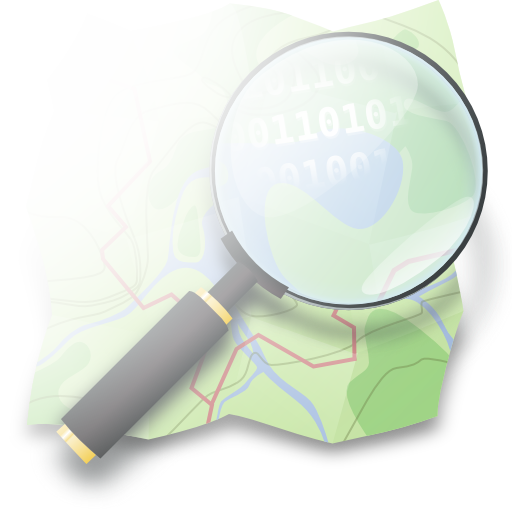
\includegraphics[height=3cm]{osm-logo-gradient.png}}

\AtBeginSection[]
{
    \begin{frame}<beamer>
        \tableofcontents[currentsection]
    \end{frame}
}

\newcommand{\notepage}[1]{
    \note{\tiny\parskip2ex
        #1 \\
    }
}

%\beamerdefaultoverlayspecification{<+->}

\begin{document}

\begin{frame}
    \titlepage
\end{frame}

\begin{frame}
    % Nur Chapter und Section ins Inhaltsverzeichnis
    \setcounter{tocdepth}{2}
    \tableofcontents
\end{frame}

\section{Allgemeines}

\begin{frame}{Was ist OpenStreetMap?}
    \pause
    \centerline{\Large OpenStreetMap ist eine freie Weltkarte}
\end{frame}

\begin{frame}{Inhalte}
    \begin{itemize}
        \item Straßen
        \item Flächen/Landnutzung
        \item Gebäude
        \item POIs
        \item Vegetation
        \item \ldots
    \end{itemize}

    \vfill

    \pause
    \centerline{Inzwischen über 550~000 User und 1~500~000~000 Objekte.}

    \vfill
\end{frame}

\notepage{
    Es existieren unzählige weiteren Informationen, z.B. Verlinkungen zu Wikipedia"=Einträgen, Geschwindigkeitsbegrenzungen, Begehungsrechte/Öffnungszeiten, TMC"=Informationen, Objekte wie Türme, Kraftwerke, Bushaltestellen, ÖPNV"=Netze, \ldots
}

\begin{frame}{Lizenz}
    \pause
    \begin{itemize}
        \item Ursprünglich: CC"=BY"=SA
        \item Seit April 2012: ODbL\footnote<2->{Open Database License}
    \end{itemize}

    \pause

    \begin{itemize}
        \item Kostenlose Nutzung der Daten
        \item Auch kommerziell
        \item Attribution (Namensnennung)
        \item Share Alike (Weitergabe unter gleichen Bedingungen)
    \end{itemize}
\end{frame}

\notepage{
    Neben der ODbL gibt es noch eine Reihe weiterer relevanter Lizenzen. Die sind am Ende dieser Folie verlinkt. Wenn man es ganz stark vereinfacht, kann man sagen: Solange du OSM als Quelle angibst, darfs du mit den Daten machen, was du willst.

    Das gilt übrigens nicht ganz für die erzeugten Tiles (sind weiterhin CC) und bereitgestellte Services: Dort gilt üblicherweise das Fair"=Use"=Prinzip. Wenn ein Produkt die OSM"=Server stark belastet, wird es gesperrt und muss die Tiles auf den eigenen Servern rendern. Änliches gilt z.B. für Read"=Only"=API"=Dienste.

    Aber was bedeutet das "`frei"' eigentlich? Beispiel: Man möchte jemandem etwas auf einer Karte in einem Dokument für das Internet zeigen. Dazu macht man einen Screenshot von Google Maps und bindet diesen inklusive Quellenangabe ein. -- Ist das erlaubt? Bei Google Maps muss man jetzt lange und umständlich die Lizenzen durchsuchen (sofern man die überhaupt schnell findet), bei OSM braucht man darüber nicht weiter nachdenken -- Quelle drunter, fertig. Es kommt also noch nichtmal auf das "`kostenlos"' ("`free as in free beer"'; die gerenderten Tiles können ggf. kostenpflichtig sein, genauso auf den Daten aufbauende Dienste, s.o.), sondern auch hauptsächlich auf das "`ohne Einschränkungen"' ("`free as in free speech"') an.

    PS: Bei Google Maps ist das übrigens soweit ich weiß für private, nicht"=kommerzielle Zwecke gestattet.

    \href{http://www.osmfoundation.org/wiki/License/Contributor\_Terms}{Contributor Terms}, \href{http://opendatacommons.org/licenses/dbcl/1.0/}{Database Contents License (DbCL)}, \href{http://opendatacommons.org/licenses/odbl/}{Open Data Commons Open Database License (ODbL)}
}

\begin{frame}{Organisation}
    \pause
    \begin{itemize}
        \item \href{http://www.osmfoundation.org/}{OpenStreetMap Foundation (OSMF)}
            \begin{itemize}
                \item 2006 Gegründet
                \item Non"=Profit"=Organisation
                \item Verwaltet Interessen von OSM
                \item Betreibt die Server und einige Dienstleistungen
            \end{itemize}
        \vfill\pause
        \item Arbeitsgruppen
            \begin{itemize}
                \item Befassen sich mit Teilaspekten
                \item Gehören zur OSMF
            \end{itemize}
            \begin{itemize}
                \scriptsize
                \item Communication Group
                \item Data Working Group
                \item License Working Group
                \item Local Chapters Working Group
                \item Technical Working Group
                \item Data Import Support Working Group
            \end{itemize}
    \end{itemize}
\end{frame}

\notepage{
    Ein so großes Projekt wie OpenStreetMap kann nicht von tausenden Beteiligten in Eigenregie verwaltet werden. Deswegen wurde die OpenStreetMap Foundation (OSMF) gegründet, welche sich mit den meisten verwaltungstechnischen Belangen von OSM befasst. Dabei ist der Grundgedankte nicht, alles zu bestimmen und Entscheidungen zu treffen, sondern zu vermitteln, Entscheidungen auszuführen und OSM dritten gegenüber zu vertreten.

    % description-Umgebung will irgendwie nicht, macht nicht fett, aber unterschiedliche Einrückungen

    \textbf{Communication Group} Pflege von OSMF"=Webseite und Kommunikationswegen, Förderung der Kommunikation

    \textbf{Data Working Group} Urheberrechtsverletzungen, Vandalismus

    \textbf{License Working Group} Erstellung der neuen Open Database License

    \textbf{Local Chapters Working Group} Lokale Vertretungen der OSMF, in Deutschland der \href{http://www.fossgis.de/}{FOSSGIS e.V.}

    \textbf{Technical Working Group} Wartung und Betrieb der Server

    \textbf{Data Import Support Working Group} Sucht weltweit nach lizenzrechtlich kompatiblen Daten und Organisiert den Import
}

\section{Geschichte}

\subsection{Die Anfänge}

\begin{frame}{Die Anfänge}
    \begin{itemize}
        \item 2004 auf der EuroFoo von Steve Coast präsentiert
        \vfill
            \begin{itemize}
                \item Alternative zu kommerziellen Karten
                \vfill
                \item Erste Beispiele und Vergleiche
                \vfill
                \item Idee zu gemeinschaftlicher Arbeit
                \vfill
                \item Grenzen von GPS
                \vfill
                \item Großes Vorhaben -- realisierbar?
                \vfill
                \item Möglicherweise mit Luftbildern, sofern freie Lizenz
                \vfill
                \item Taxi, Kuriere und Co. als Quelle?
            \end{itemize}
    \end{itemize}
    \vfill
\end{frame}

\notepage{
    Das Euro Foo Camp fand im August 2004 in den Niederlanden statt. Weitere Informationen:\\
    \url{http://wiki.oreillynet.com/eurofoo/index.cgi}
}

\subsection{Der Aufstieg}

\begin{frame}{Der Aufstieg}
    \begin{figure}
        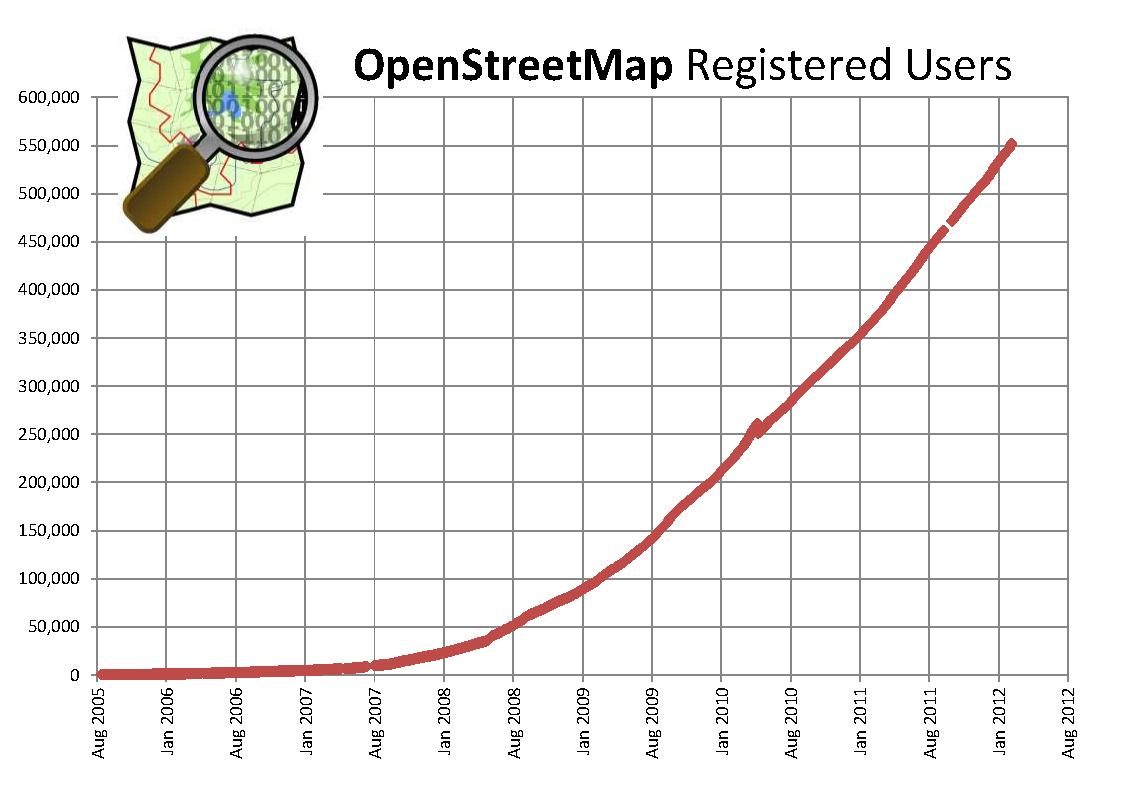
\includegraphics[height=6.5cm]{Osmdbstats1_users.png}
    \end{figure}
\end{frame}

\begin{frame}{Der Aufstieg}
    \begin{figure}
        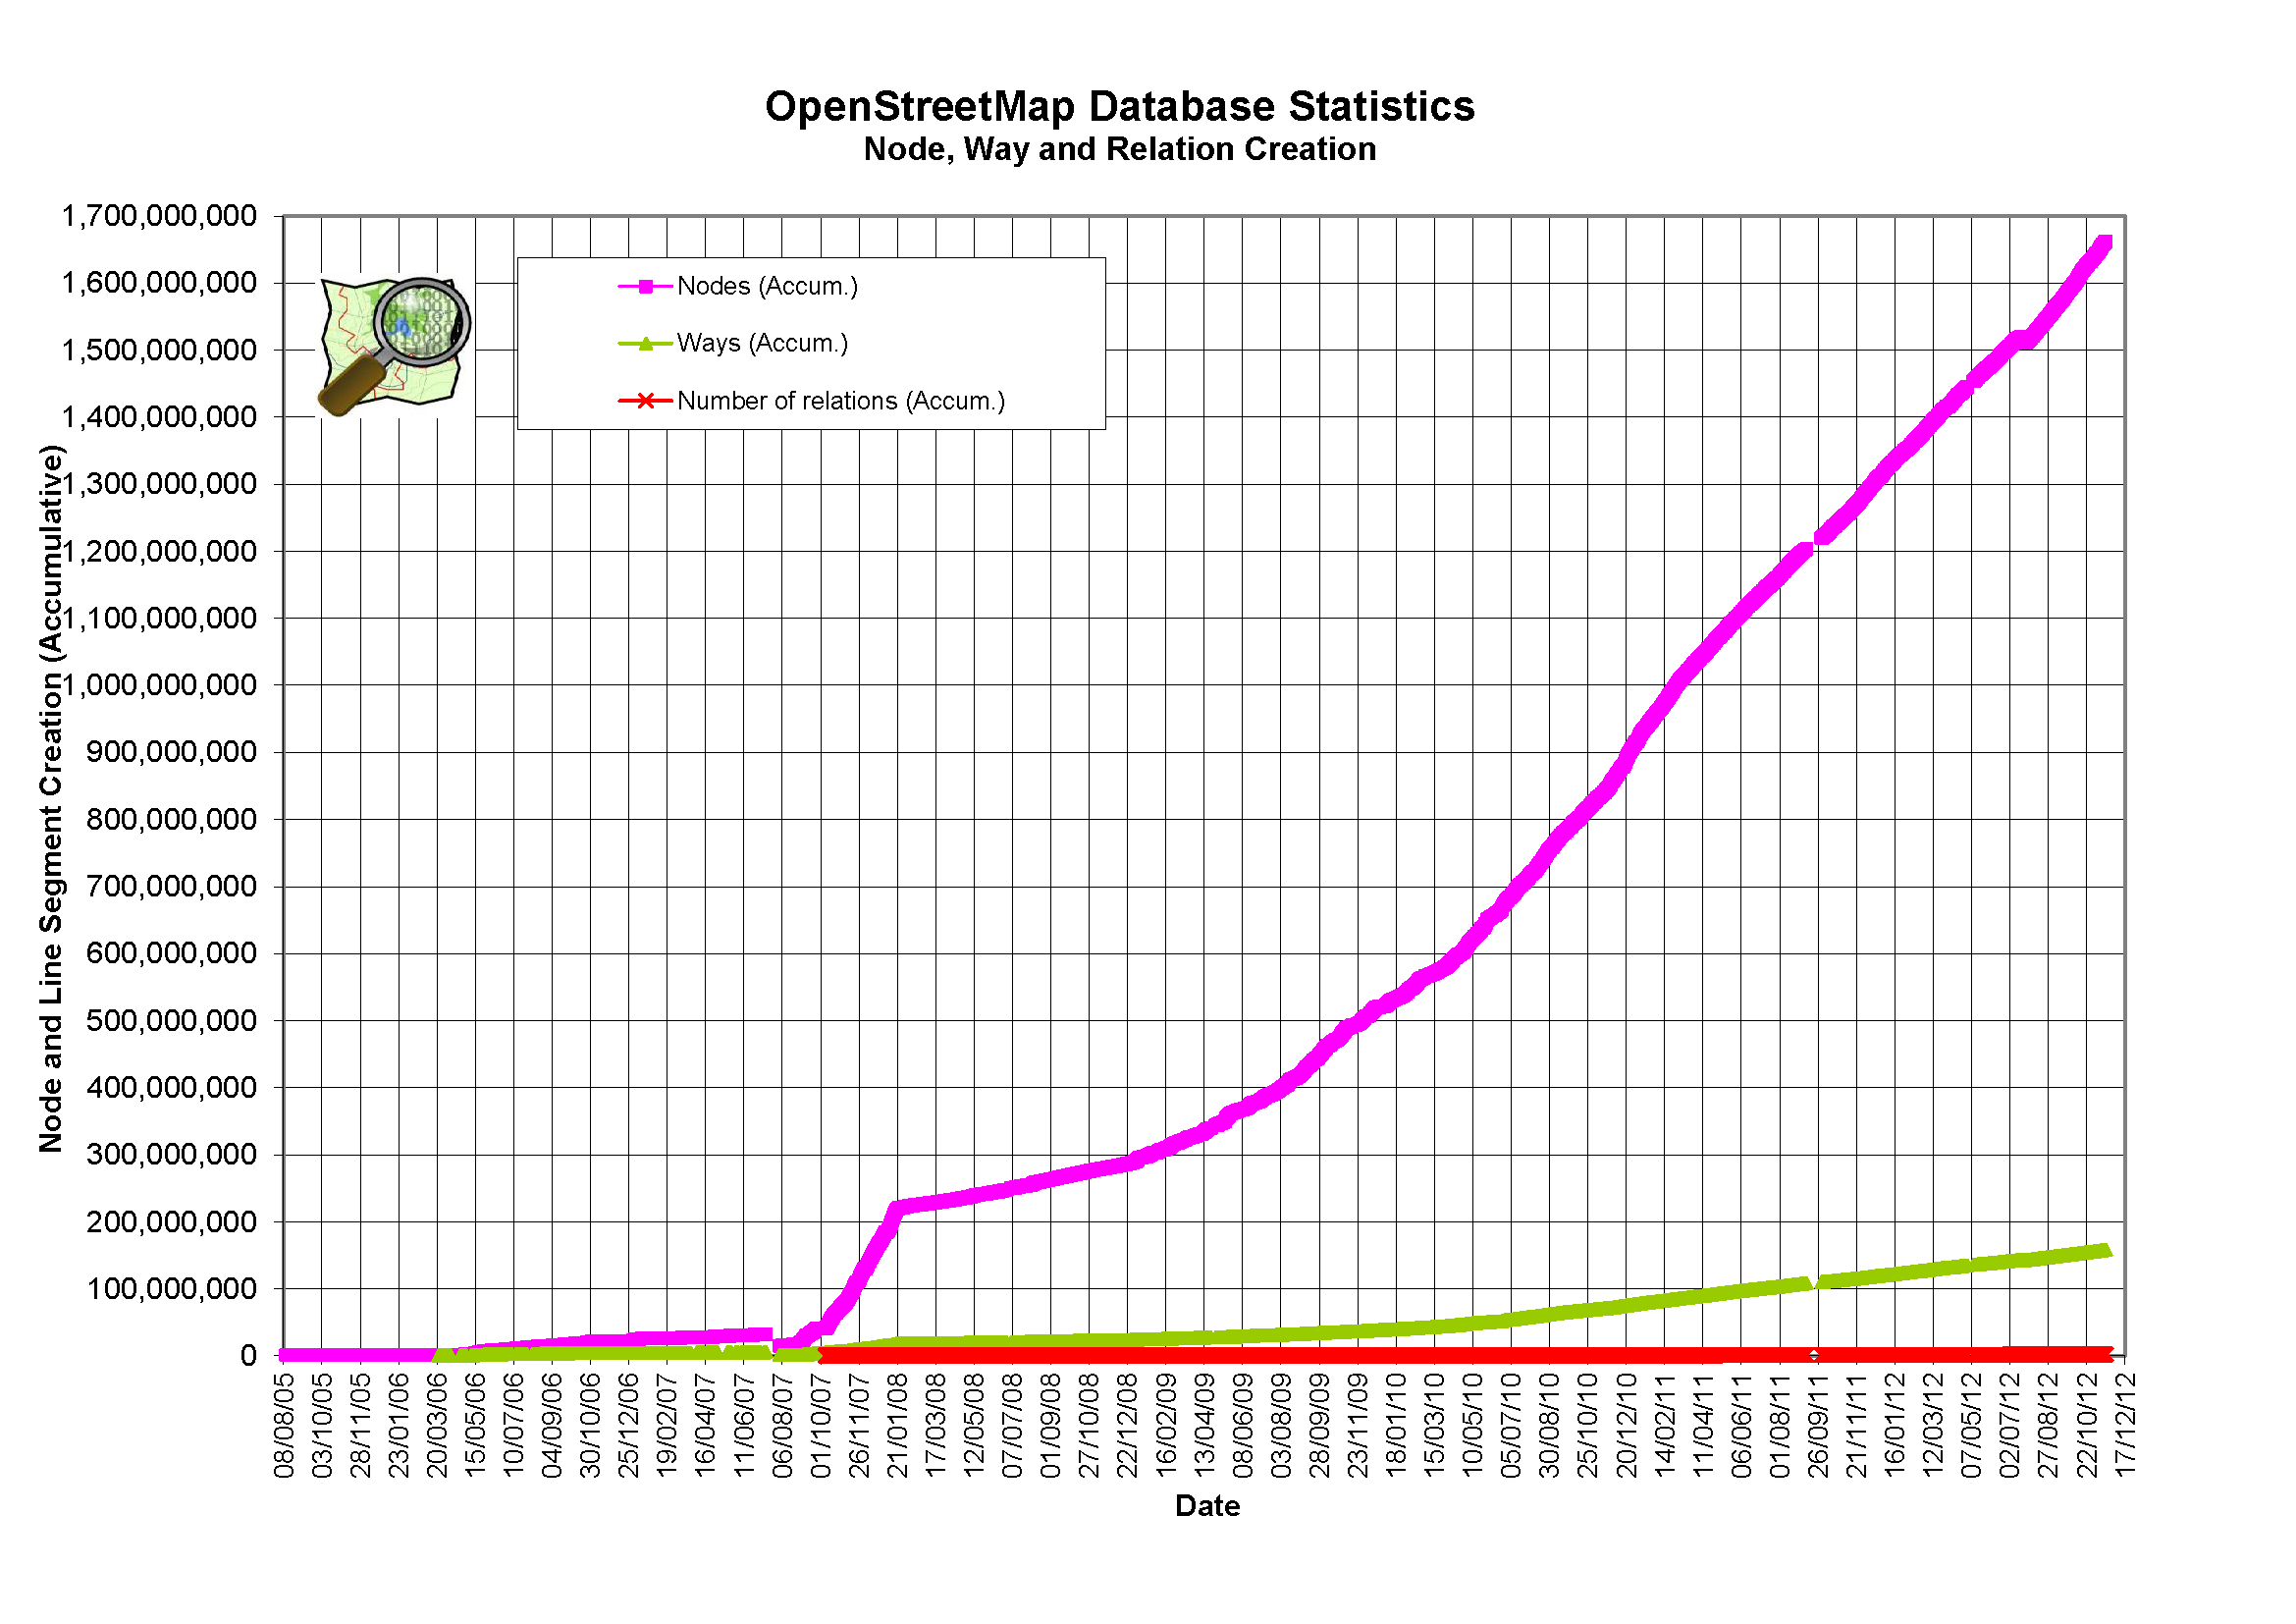
\includegraphics[height=6.5cm]{Osmdbstats2.png}
    \end{figure}
\end{frame}

\notepage{
    Der kleine Sprung im August 2007 kommt daher, dass zuvor auch gelöschte Objekte gezählt wurden, danach nur noch vorhandene. Der steile Anstieg wird weiter unten erklärt.

    Noch mehr Statistiken gibt es hier: \url{http://j.mp/OSM-stats}

    Über Google finden sich auch noch sehr viele weitere, teils ziemlich spezielle Statistiken.
}

\subsection{Der Lizenzwechsel}

\begin{frame}{Der Lizenzwechsel}
    \pause
    \begin{itemize}
        \item CC nicht für Daten geeignet
        \item Betrachtet jeden Einzelnen und nicht das Gesamtwerk
    \end{itemize}

    \pause

    \begin{itemize}
        \item Neue Lizenz muss her! $\rightarrow$ \textbf{ODbL}
    \end{itemize}

    \pause

    \begin{itemize}
        \item Unterschiedliche Meinungen
        \item Langwieriger Umstellungsprozess (u.a. jeder muss zustimmen/ablehnen)
        \item Schrittweise Umstellung seit 1. April 2012
    \end{itemize}

    \pause

    \begin{itemize}
        \item Letztendlich: Großer Datenverlust
        \item Aber auch neue Möglichkeiten!
    \end{itemize}
\end{frame}

\notepage{
    In vielen Ländern waren die Daten bisher nicht durch die CC geschützt (z.B. USA). CC stützt sich nur auf Urheberrecht und bei OSM ist die Schöpfungshöhe oft nicht ausreichend. Außerdem bezieht sich die CC auf jeden einzelnen Bearbeiter, wenn man die Karten nutzt, müsste also jeder betroffene Bearbeiter (ggf. tausende!) aufgrund der Attribution genannt werden.

    Es gab viele diskutierte Lizenzen, fertige und neue. Gab viele Argumente dafür und dagegen, letztendlich wurde aus den Kompromissen diese neue Lizenz erstellt.
    
    Die Bezogenheit auf den Einzelnen der CC ist auch der Grund, warum jetzt jeder einzeln zustimmen muss. Die Zustimmung ist bei Anmeldung seit Mai 2010 Pflicht bzw. seit April 2011 für alte Accounts, wenn man etwas bearbeiten will. Wer nicht zustimmt, dessen Daten müssen gelöscht werden. Das ist ein komplizierter Prozess, denn: Wann sind alte Bearbeitungen nicht mehr relevant? Wem gehört die Geometrie, wem die Eigenschaften? Wie kann man einer Inkonsistenz der Daten entgegenwirken (z.B. Nodes an Kreuzungen)?

    Möglichkeiten: OSMF kann für alle entscheiden, zukünftig kein Datenverlust mehr, umfangreicherer Schutz der Daten, da nicht nur auf Urheberrecht gestützt

    Die Umstellung begann mit einem Wechsel in einen Read"=Only"=Modus für einige Tage, während der Datenbankserver getauscht wurde. Anschließend sperrt ein Bot Stück für Stück im Live"=Betrieb Daten mit Lizenzinkompatibilität, man kann die Daten also nicht mehr über die normale API herunterladen und sie sind auch nicht in den Planet"=Files.

    Weitere Infos: \href{http://wiki.openstreetmap.org/wiki/Openi\_Data\_License/Implementation\_Plan}{Implementation Plan}, \href{http://wiki.openstreetmap.org/wiki/Open\_Database\_License/Changes\_in\_the\_API}{Changes in the API}
}

\section{Technik}

\subsection{Infrastruktur}

\begin{frame}{Infrastruktur / Server}
    \begin{itemize}
        \item Über 20 Server in Betrieb
        \vfill
        \item An zwei Standorten in England
        \begin{itemize}
            \item University College London
            \item Imperial College London
        \end{itemize}
        \vfill
        \item Kleinere Komponenten weltweit verteilt
        \vfill
        \item Finanziert über Spenden
        \vfill
        \item Transparente Administration (Vorgänge werden öffentlich protokolliert, ständige Statusübersicht z.B. über Munin)
    \end{itemize}
    \vfill
\end{frame}

\notepage{
    Die Server sind alle nach Drachen benannt, in Anlehnung an "`Here be dragons"', was früher auf Karten für unentdecktes Land stand.

    Für gewöhnlich sind die Server zu Spitzenzeiten stark ausgelastet. Gerade bei den Tile"=Servern merkt man, dass diese sehr lange Antwortzeiten haben. Dies liegt daran, dass viele -- zum Teil auch größere -- Dienste die Tiles für ihre eigenen Seiten nutzen (generierung von Offline"=Raster"=Karten, Online"=Karten auf viel besuchten Seiten oder in mobilen Anwendungen, \ldots). Einige dieser Dienste wurden bereits unter Hinweis auf die Nutzungsbedingungen gesperrt (mit Hilfe des Referers).

    Interessante Übersicht zu den Servern: \url{http://wiki.openstreetmap.org/wiki/Servers}
}

\begin{frame}{Datenzugriff}
    \pause
    \begin{block}{Export}
        \begin{itemize}
            \item Wöchentliche komplette Exporte (Planet"=Files), tägliche/minütliche Diffs
            \item Bereitgestellt auf diversen Mirrors
            \item Programm zur lokalen Verwaltung: \href{http://wiki.openstreetmap.org/wiki/Osmosis}{Osmosis}
        \end{itemize}
    \end{block}

    \pause

    \begin{block}{API}
        \begin{itemize}
            \item Für kleinere (ggf. spezielle) Abfragen
            \item Mehrere Dienste von verschiedenen Anbietern
            \item API von osm.org auch schreibender Zugriff
        \end{itemize}
    \end{block}
\end{frame}

\notepage{
    Weitere Informationen zu den Planet Files und Mirrors: \url{http://wiki.openstreetmap.org/wiki/Planet.osm}

    Es gibt einige allgemeine und viele spezielle APIs (nur bestimmte Daten, komplexe Ausschnitte, \ldots). Am wichtigsten ist jedoch die API von openstreetmap.org (aktuell Version 0.6), denn darüber lassen sich eigene Daten hochladen. Allerdings werden Anfragen ab einer gewissen Größe blockiert. Weitere Informationen zur OSM"=API: \url{http://wiki.openstreetmap.org/wiki/Api}
}

\subsection{Karten}

\begin{frame}{Renderer}
    \pause
    \begin{itemize}
        \item Etliche Renderer
        \item Unterschiedliche Ziele
        \item Teilweise eigene Style"=Definitionen möglich
    \end{itemize}

    \begin{itemize}
        \item Erzeugen aus (Vektor"=)Daten ein Rasterbild (üblicherweise png oder gif)
    \end{itemize}

    \pause

    \begin{itemize}
        \item Mapnik überwiegend für Webkarten
        \item Osmarender im tiles@home"=Netzwerk (eingestellt)
        \item In Editoren für lokale Betrachtung
    \end{itemize}
\end{frame}

\begin{frame}{Slippy Map}
    \begin{itemize}
        \item Scrollbare Karte in Webseiten eingebettet
        \vfill
        \item Auslieferung als Tiles (quadratische Bilder)
        \vfill
        \item Über spezielles Koordinatensystem adressiert
        \vfill
        \item Einfache URL: \texttt{\footnotesize http://\{a|b|c\}.tile.openstreetmap.org/zoom/x/y.png}
        \vfill
        \item Parameter: \texttt{/status} und \texttt{/dirty}
    \end{itemize}
    \vfill
\end{frame}

\notepage{
    Als Technologie für die Webkarten wird wie üblich für dynamische Inhalte AJAX eingesetzt, also eine Kombination aus html und JavaScript, welches Daten bei Bedarf nachlädt. Außerdem werden mit JavaScript Maus"= und Tastatureingaben abgefangen um die Karte zu bewegen / zoomen.

    Die Karten werden wie üblich in Form von Tiles (quadratische Bilder) ausgeliefert. Diese werden über eine einfache URL abgerufen, welche Parameter für ein (clientseitiges) Balancing, Zoom, x und y Position enthält. Dieses Format ist meines Wissens nach ein (Quasi"=)Standard und wird von vielen Diensten eingesetzt.

    Es können zwei weitere Parameter am Ende (hinter \texttt{.png}) übergeben werden: \texttt{/status} liefert in Textform Informationen z.B. über die Renderzeit. \texttt{/dirty} markiert das Tile als "`veraltet"' und veranlasst eine Einreihung in die Renderqueue.
}

\begin{frame}{Map Rendering}
    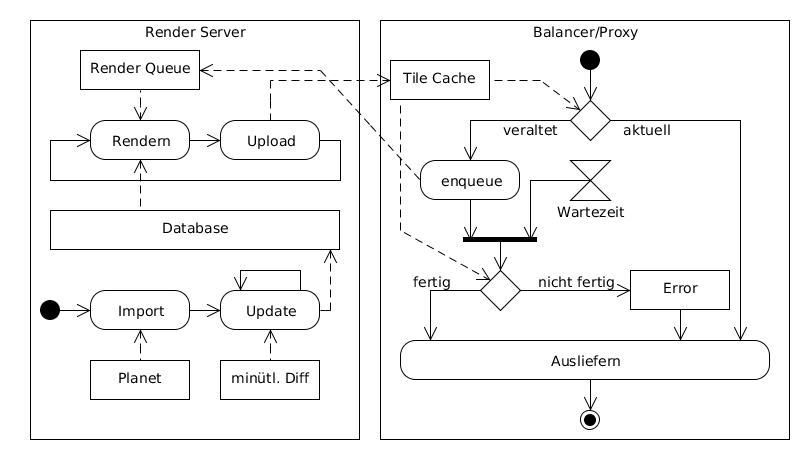
\includegraphics[height=6cm]{Renderablauf.png}
\end{frame}

\notepage{
    Grundsätzlich muss man zwei Server("=Cluster) trennen: Den Render"=Server und den Proxy"=Server.

    Auf dem Render"=Server wird alle paar Monate die Datenbank komplett aus den Planet"=Files übernommen. Zwischenzeitlich wird sie nur über die minütlichen Diffs aktualisiert, was öfters zu kleineren Problemen führt (inkonsistente Daten und dadurch fehlerhaft gerenderte Gebiete).\\
    Außerdem existiert dort ein Render"=System, welches ständig (und möglichst voll ausgelastet) eine Queue mit Renderaufträgen abarbeitet. Diese werden anschließend auf einen Proxy"=Server hochgeladen.

    Beim Proxy"=Server gehen Anfragen der Nutzer nach Tiles ein. Zuerst wird überprüft, ob im Tile"=Cache ein ausreichend aktuelles Tile vorhanden ist. Ist dies der Fall, kann es sofort ausgeliefert werden. Andernfalls wird es in die Renderqueue eingereiht und einen Moment gewartet (wenige Sekunden). Wurde das Tile bis dahin erzeugt, kann es ausgeliefert werden. Wenn nicht, dann wird entweder ein altes oder (wenn das Tile noch nie gerendert wurde) ein Fehlerbild ausgeliefert.
}

\subsection{Datenstrukturen}

\begin{frame}{Drei Datentypen}
    \pause
    \begin{itemize}
        \item Node
            \begin{itemize}
                \item Einfacher Punkt
            \end{itemize}
        \vfill\pause
        \item Way
            \begin{itemize}
                \item Folge aus Punkten
                \item Geschlossener Weg = Fläche\footnote<3->{Kann durch Tags beeinflusst werden}
                \item Sind gerichtet
            \end{itemize}
        \vfill\pause
        \item Relation
            \begin{itemize}
                \item Menge aus anderen Objekten
                \item Sind geordnet
            \end{itemize}
    \end{itemize}
\end{frame}

\notepage{
    Der Punkt bzw. Node ist der elementarste Datentyp in einer Geo"=Datenstruktur. Er beschreibt eine Position im Raum. Für einfache 2D"=Zwecke wird dafür üblicherweise ein Koordinatenpaar in Bezug zu einem Referenzsystem genutzt. Bekannt (und in fast allen Anwender"=Geosystemen genutzt) ist das WGS84 (\href{http://de.wikipedia.org/wiki/World\_Geodetic\_System\_1984}{World Geodetic System 1984}). Das ist ein spannendes Thema, würde den Rahmen dieses Vortrags aber überschreiten.

    Wege sind dann die logische Fortsetzung von Punkten. Sie sind eine Liste von Punkten, die geordnet und gerichtet ist. Geordnet ist selbstverständlich, sonst würde ein Weg anders verlaufen, denn es müssen ja nicht immer Punkte mit dem kleinsten Abstand verbunden werdne. Gerichtet, damit z.B. Einbahnstraßen ermöglicht werden. In den Datenstrukturen von OSM wird mit Wegen auch ein weiterer wichtiger Basistyp implementiert: die Fläche. Ist nämlich ein Punkt sowohl Anfang als auch Ende eines Weges, so wird dies als Fläche interpretiert. Für Renderer und teilweise auch Auswertungen kann man dies mit Tags überschreiben und so z.B. einen Ring als Kreisverkehr oder eine offene Figur als Fläche darstellen (letzteres macht eigentlich keinen Sinn, es werden dann aber die Endpunkte mit einer virtuellen Kante verbunden).

    Relationen beschreiben Gruppen und Beziehungen zwischen Objekten. Dadurch kann man z.B. Multipolygone erzeugen (also Flächen mit "`Löchern"'), aber auch zusammengehörige Ortsteile, Gebäudegruppen, Buslinien etc.
}

\begin{frame}{Tags}
    \begin{itemize}
        \item \texttt{<name>=<value>}
        \vfill
        \item Theoretisch frei wählbar
        \vfill
        \item Empfohlene Tags im Wiki dokumentiert
        \vfill
        \item Aktuell mehrere tausend, teilweise heftig diskutiert
        \vfill
        \item Abstimmungsverfahren für neue Tags
    \end{itemize}
    \vfill
\end{frame}

\notepage{
    Tags sind ein umfangreich diskutiertes Thema. Es gibt zwar Richtlinien, die über Vorschlags"= und Abstimmungsverfahren von der Community festgelegt werden, aber vieles wird unterschiedlich ausgelegt und jeder kann die Tags nach Belieben einsetzen. Es gibt also keinen fest definierten Objektartenkatalog wie z.B. \href{http://de.wikipedia.org/wiki/Amtliches\_Topographisch-Kartographisches\_Informationssystem}{ATKIS} und somit einige Probleme (redundante Tags, Fehler beim Rendern und Auswertung, \ldots).

    Es gibt in der Wiki einige hilfreiche Übersichtsseiten für den Anfang:

    \begin{itemize}
        \item \url{http://wiki.openstreetmap.org/wiki/DE:Map\_Features}
        \item \url{http://wiki.openstreetmap.org/wiki/DE:Howto\_Map\_A}
    \end{itemize}
}

\begin{frame}{Objekte}
    \center{
        Datentyp\\
        +\\
        Tags\\
        +\\
        \ Versionierung\footnote{bestehend aus Datum, Benutzer, Changeset}
    }

    \vfill\pause

    \begin{itemize}
        \item Changesets um Änderungen zusammenzufassen
    \end{itemize}

    \vfill
\end{frame}

\notepage{
    Changesets sind genaugenommen auch ein Datentyp, nur dass er nichts mit den Geodaten zu tun hat. Er ist ähnlich wie eine Relation, allerdings ohne Ordnung, hat aber wie alle anderen Objekte Tags und einen Benutzer.
}

\section{Verwendung}

\subsection{Nutzung}

\begin{frame}{Nutzung}
    \begin{itemize}
        \vfill
        \item Web: freie Alternative zu Google Maps \& Co.
        \vfill
        \item Alternative zu kommerziellen offline Karten (z.B. Garmin GPS, Mapsource, qlandkarte gt, \ldots)
        \vfill
        \item Offline"=Routing mit Vektorkarten
        \vfill
        \item Diverse Analysen: Waldanteil, Straßendichte, \ldots
        \vfill
        \item Zeitvertreib
        \vfill
    \end{itemize}
\end{frame}

\notepage{
    Geodaten finden in sehr vielen Bereichen Verwendung. Privat z.B. in Blogs oder zur Navigation und Orientierung, in der Wissenschaft usw. Oft gibt es dann halt das Problem mit der Lizensierung: Was darf ich machen? Wenn ich das jetzt einbaue und später das fertige Produkt anderweitig werwenden will -- darf ich das dann immer noch? Diese Fragen stellen sich halt nicht mit OSM (s.o.) und je detaillierter und umfangreicher die Daten werden, desto mehr kann man damit machen. Einfach mal versuchen, für eine Woche oder so ausschließlich freie Geodaten zu nutzen.

    Einer der wichtigsten Punkte ist der Zeitvertreib und der Wille, freie Daten zu fördern. Letztendlich erfolgt fast alles bei OpenStreetMap auf freiwilliger, ehrenamtlicher Grundlage. Das Mappen kann eine Menge Spaß machen und man lernt seine Umgebung gut kennen. Sogar im Urlaub lassen sich Notizen machen und diese später in OSM hinzufügen. So kann man den Urlaub noch etwas aufarbeiten (und sich erinnern).
}

\subsection{Datenquellen}

\begin{frame}{Datenquellen}
    \invisible<3-5>{
        \begin{itemize}
            \item<2-> GPS
                \begin{itemize}
                    \item Tracks
                    \item Einzelne Messpunkte
                \end{itemize}
            \vfill
            \item<6-> Luftbilder
                \begin{itemize}
                    \item Yahoo
                    \item Bing
                    \item AeroWest
                \end{itemize}
            \vfill
            \item<7-> Datenspenden / Public Domain Quellen
                \begin{itemize}
                    \item AND Automotive Navigation Data Niederlande (2007)
                    \item Gebäudeumrisse Katasteramt Rostock (2008)
                    \item TIGER USA (2007)
                \end{itemize}
            \vfill
            \item<8-> Ortskenntnisse
        \end{itemize}
    }

    \only<3>{
        \begin{textblock}{10}(3,4)
            \centering 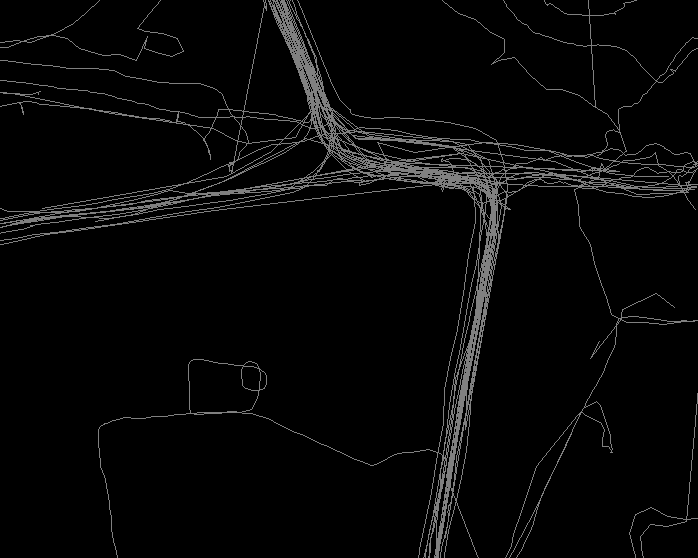
\includegraphics[height=6cm]{gps-tracks.png}
        \end{textblock}
    }
    \only<4>{
        \begin{textblock}{10}(3,4)
            \centering 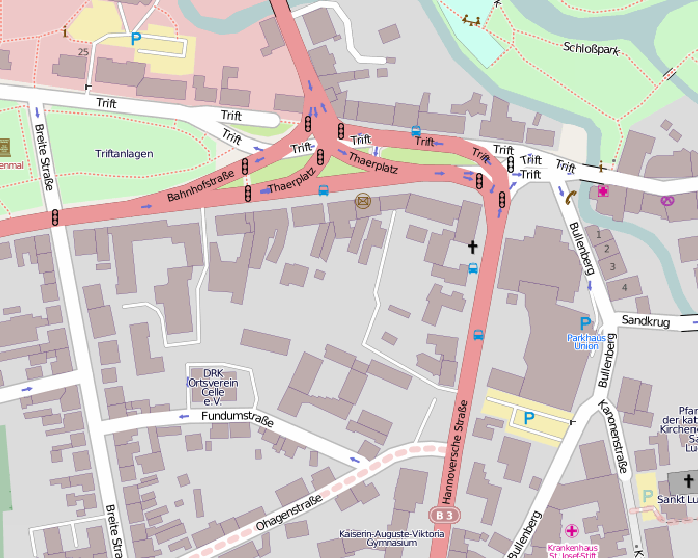
\includegraphics[height=6cm]{gps-tracks_mapnik.png}
        \end{textblock}
    }
    \only<5>{
        \begin{textblock}{10}(3,4)
            \centering 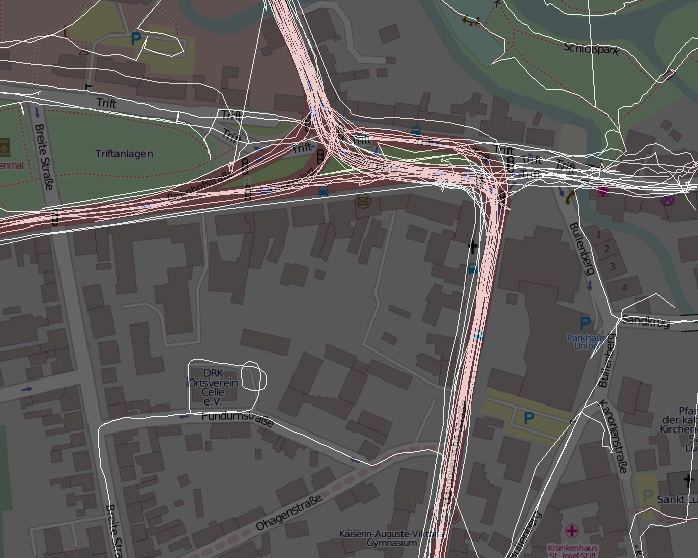
\includegraphics[height=6cm]{gps-tracks_overlay.png}
        \end{textblock}
    }
\end{frame}

\notepage{
    An den drei Bildern sieht man gut, welche Informationen man aus den GPS"=Tracks gewinnen kann und welche nicht. Man kann grob erkennen, wo große Straßen verlaufen. Allerdings weiß man nicht genau, wie die Straße beschaffen ist (breit, befestigt, Fußgängerzone, \ldots).\footnote{Die Uni Hannover hat dazu interessante Forschungsprojekte, siehe \href{http://www.ikg.uni-hannover.de/index.php?id=648}{hier}.} Auch hat das GPS eine gewisse Abweichung (5-50 Meter), das kann man auf zwei Arten kompensieren: Viele Tracks mitteln oder selbst erstellen und mögliche Fehler notieren. Bei den ganzen fremden Tracks sieht man auch, dass einige Fehler haben und einen Sprung machen -- da ist aber gar kein Weg! Viele Straßen sind auch gar nicht mit drin und wenn, dann nur mit ganz wenigen (fremden) Tracks, kann man also nichts mit anfangen. Auch weiß man natürlich die Straßennahmen nicht.

    Deswegen nimmt man immer häufiger Luftbilder. Die haben allerdings den Nachteil, dass sie schwer (unter einer freien Lizenz) zu bekommen sind und verzerrt sein können. Am besten alle paar hundert Meter mit dem GPS mehrere Messungen durchführen und das Bild daran ausrichten. Urspünglich durften Yahoo und Landsat Bilder genommen werden. Dann hat Microsoft sie mit ihrem Produkt "`Bing"' freigegeben zum Abzeichnen. Mit dem Projekt "`Wissenswert"' dürfen von Juli 2011 bis Juli 2012 Luftbilder (5-10 cm Auflösung!) verwendet werden. Weitere Informationen: \url{http://wiki.openstreetmap.org/wiki/DE:WissensWert/Luftbilder}

    Außerdem werden gelegentlich freie bzw. gespendete Daten importiert. Große Beispiele sind die drei oben erwähnten, aber es gibt noch Dutzende weitere. Darunter auch kleinere, wie z.B. alle Standorte der Kette "`Rossmann"'. Durch AND und TIGER haben die USA und Niederlande eine großflächige Abdeckung bekommen. Weiter oben kann man diesen Sprung in der Statistik sehen, es scheint auch so, als wenn dadurch OSM sehr viel populärer wurde. Zumindest in den USA wird deswegen aber nicht so viel gemappt ("`Gibt doch schon alles."' und wenn was falsch ist / fehlt, dann beschweren sich die Leute nur). \url{http://wiki.openstreetmap.org/wiki/Import}

    Das Wichtigste sind aber Ortskenntnisse. Straßenschilder, örtliche Besonderheiten, Abbiegebeschränkungen, Hindernisse, Straßennamen, Hausnummern, \ldots
}

\subsection{Bearbeitung}

\begin{frame}{Bearbeitung}
    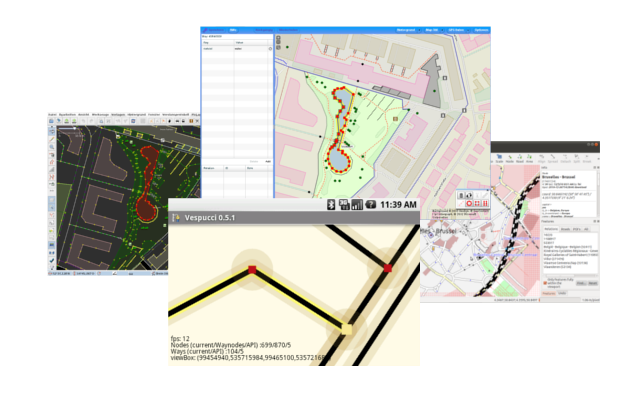
\includegraphics[height=6cm]{editor-collage.png}
\end{frame}

\begin{frame}{Bearbeitung}
    \begin{itemize}
        \item Vielfältige Möglichkeiten
        \vfill\pause
        \item Desktopanwendungen, Apps, Scripts, \ldots
        \vfill\pause
        \item Zwei Editoren haben sich durchgesetzt:
            \begin{itemize}
                \item Potlatch (Browser)
                \item JOSM (standalone)
            \end{itemize}
    \end{itemize}
\end{frame}

\notepage{
    Durch die gute Dokumentation und den einfachen Aufbau von Datenformat und API gibt es eine Vielzahl von Scripts und Programmen. Bots validieren und korrigieren Daten, einfache Webinterfaces ermöglichen das Bearbeiten bestimmter Attribute (z.B. \href{http://wheelmap.org/}{Wheelmap}, \href{http://yapis.geoclub.de/}{YAPIS}), mit grafische Editoren können komplexe Situationen modelliert werden.

    Im Folgenden soll auf lediglich zwei weit verbreitete Editoren eingegangen werden: Potlatch als webbasierte Lösung und JOSM als Desktopanwendung.
}

\subsubsection{Potlatch}

\begin{frame}{Potlatch}
    \begin{figure}
        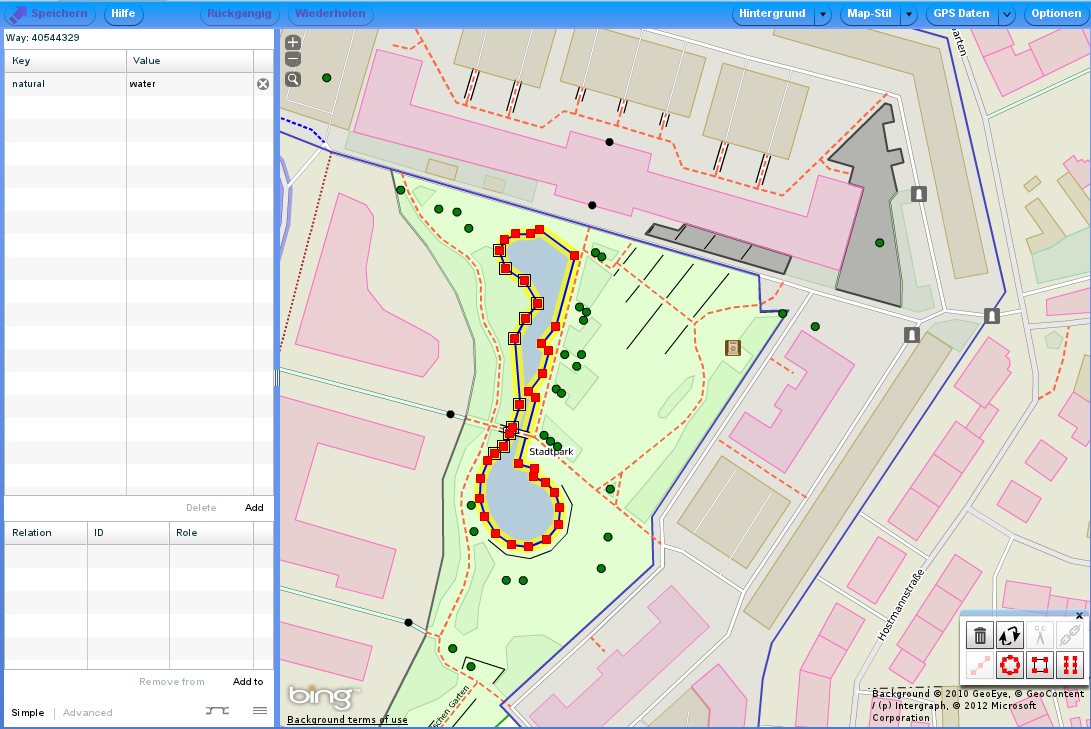
\includegraphics[height=6.5cm]{potlatch.png}
    \end{figure}
\end{frame}

\begin{frame}{Potlatch}
    \begin{block}{Vorteile}
        \begin{itemize}
            \item Wenige Werkzeuge, einfache Bedienung
            \item Ohne große Vorbereitung einsatzbereit
        \end{itemize}
    \end{block}
    
    \begin{block}{Nachteile}
        \begin{itemize}
            \item Flash (ausschließlich Adobe)
            \item Funktionsumfang begrenzt
        \end{itemize}
    \end{block}
\end{frame}

\notepage{
    Aufruf direkt auf \url{http://www.openstreetmap.org} über den Bearbeiten"=Tab.
}

\subsubsection{JOSM}

\begin{frame}{JOSM}
    \begin{figure}
        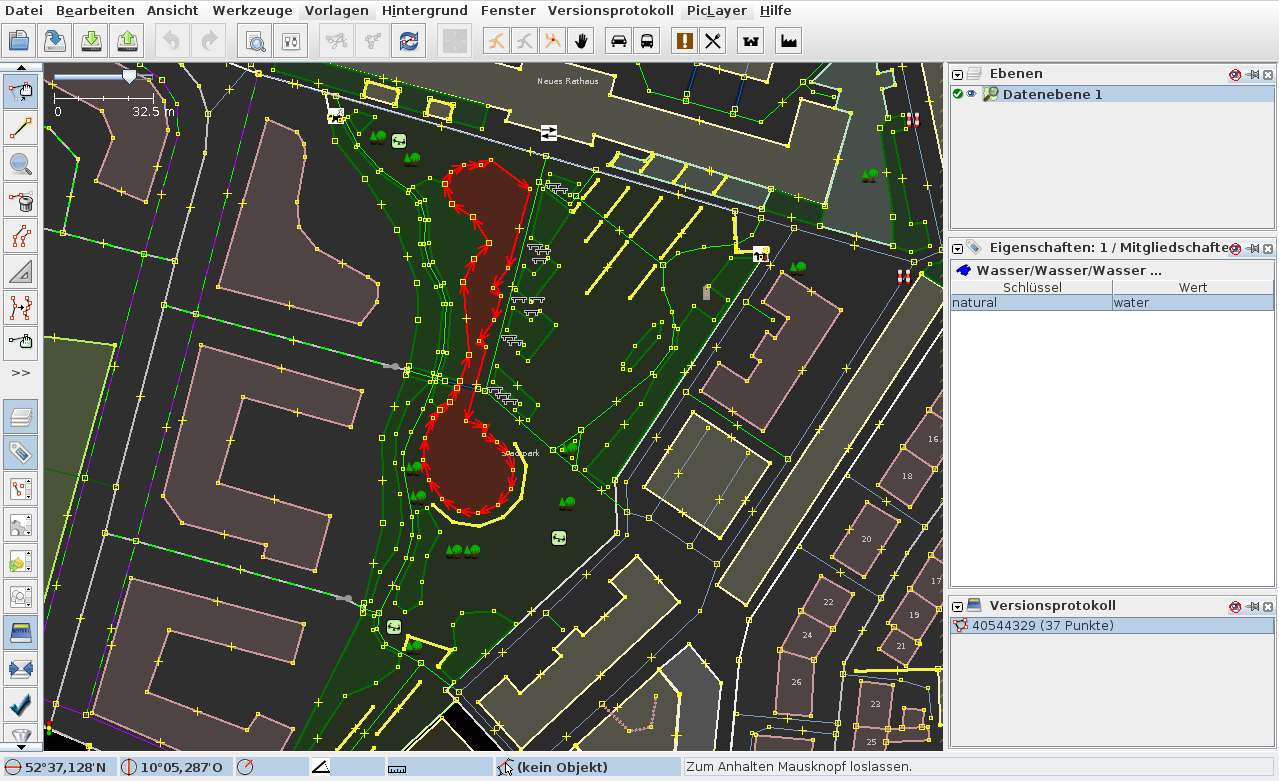
\includegraphics[height=6.5cm]{josm.png}
    \end{figure}
\end{frame}

\begin{frame}{JOSM}
    \begin{block}{Vorteile}
        \begin{itemize}
            \item Java $\rightarrow$ plattformunabhängig
            \item Viele Werkzeuge
            \item Erweiterbar durch Dutzende Plug"=Ins
            \item Speichern / Laden
        \end{itemize}
    \end{block}
    
    \begin{block}{Nachteile}
        \begin{itemize}
            \item Lange Einarbeitungszeit
        \end{itemize}
    \end{block}
\end{frame}

\notepage{
    \url{http://josm.openstreetmap.de/}
}

\section*{Mitmachen}

\begin{frame}{Ja, ich will mitmachen!}
    \pause
    \begin{itemize}
        \item Bei OSM \href{https://www.openstreetmap.org/user/new}{anmelden}
        \vfill\pause
        \item Gebiet auf der Karte wählen, oben auf "`Bearbeiten"' und dann auf "`Potlatch 2"' klicken\\
            \vfill\pause
            \hspace{1cm}\textbf{oder}
        \vfill
        \item JOSM mit all seinen Vorteilen nutzen
    \end{itemize}

    \pause
    \begin{alertblock}{}
        \centering Praxis, Übung, Ausprobieren und Spaß haben!
    \end{alertblock}
\end{frame}

\section*{Anhang}

\begin{frame}
    \begin{block}{Erstellt mit freier Software}
        \begin{itemize}
            \item \LaTeX
            \item GIMP, UMLet
            \item Ubuntu
        \end{itemize}
    \end{block}
    
    \begin{block}{Lizenz}
        CC"=BY"=NC"=SA
    \end{block}
    
    \begin{block}{Quellen}
        \begin{itemize}
            \item \url{http://openstreetmap.org/}
            \item \url{http://wiki.openstreetmap.org/}
        \end{itemize}
    \end{block}
\end{frame}

\end{document}

